\section{Experiments}
\label{sec:experiments}

\subsection{The reduced norm of basis elements before ideal multiplication}
\label{subsec:exp-basis}

\paragraph{Goal.}
In order to derive a clean upper bound for ideal multiplication, one first needs to control over the reduced norms of the basis elements of the ideals that appear \emph{before} the multiplication step. The purpose of this experiment is therefore to estimate, for each relevant ideal-generation procedure, how large the reduced norm of a basis element can be relative to the reduced norm of the ideal itself.

\paragraph{Experimental setting.}
For each sampled left $\calO_0$-ideal \(I=\langle \alpha_1,\alpha_2,\alpha_3,\alpha_4\rangle\), we computed
\[
R(I) \;:=\; \frac{\max_{1 \le i \le 4} \nrd(\alpha_i)}{\nrd(I)},
\]
where \(\{\alpha_1,\alpha_2,\alpha_3,\alpha_4\}\) denotes the natural lattice basis used in the implementation, and we checked whether \(R(I)\) exceeds the prescribed threshold \(\frac{64p^2}{\pi^2}\nrd(I)\) used in the multiplication analysis. The experiment was carried out for all concrete SQIsign parameter sets of each security parameter $\lambda\in\{128,192,256\}$, with \(10{,}000\) independent trials for each algorithm and for each parameter set. In accordance with the actual protocol path immediately preceding ideal multiplication, we excluded the standalone call Algorithm~\ref{alg:RandomIdealGivenNorm}, since its output is not used directly as an input to the multiplication step, but we retained Algorithm~\ref{alg:RandomEquivalentPrimeIdeal} applied after this call. Thus, the tested procedures were as follows:
\begin{itemize}
\item \textsf{RandomEquivalentPrimeIdeal}$\circ$\textsf{RandomIdealGivenPrimeNorm}
\item \textsf{RandomIdealGivenNorm}
\item \textsf{KernelDecomposedToIdeal}
\end{itemize}
% for signing-side composite inputs \(N\), and \(\textsf{KernelDecomposedToIdeal}\).

\paragraph{Result.}
Across all \(10{,}000\) trials for every included algorithm and every parameter set, we did not observe a single sampled ideal whose basis contained an element with reduced norm exceeding the chosen threshold $\frac{64p^2}{\pi^4}\nrd(I)$. Hence, it provides strong heuristic evidence that the ideals entering the multiplication step satisfy the basis-norm bound required for the derivation of the ideal-multiplication estimate.

% \subsection{The output distribution of RandomIdealGivenPrimeNorm}
% \label{subsec:exp-RandomIdealGivenNorm}

% \paragraph{Goal.} The purpose of this experiment is to provide heuristic evidence that the modified sampler in Algorithm~\ref{alg:RandomIdealGivenNorm} outputs left $\mathcal O_0$-ideals of norm $N$ according to the uniform distribution. Since the algorithm produces an ideal of the form
% \[
% J'=\mathcal O_0\langle g,N\rangle,
% \qquad
% g=\gamma\beta \bmod N,
% \]
% where $N$ is prime, it is natural to study the induced distribution on the corresponding projective label in $\mathbb P^1(\mathbb F_N)$. Uniformity of these labels is the finite, directly testable consequence of the target claim.

% \paragraph{Experimental setting.} For each security parameter $\lambda\in\{128,192,256\}$, we used the SQISign NIST-I/III/V base prime $p$ and set
% \[
% N_\lambda:=\min\{\ell>\,2^{4\lambda}:\ \ell \text{ prime and } \ell\equiv 1 \pmod 4\}.
% \]
% This yielded instances with
% \[
% (\mathrm{bits}(p),\mathrm{bits}(N))=(251,513),\ (383,769),\ (505,1025)
% \]
% for $\lambda=128,192,256$, respectively. For each $\lambda$, we generated $20$ independent runs, each consisting of
% \[
% n_{\mathrm{samp}}=100{,}000
% \]
% samples from Algorithm~\ref{alg:RandomIdealGivenNorm}. Because exact testing on all $N+1$ projective labels is infeasible at these cryptographic sizes, we used a bucketed goodness-of-fit test.

% More precisely, for each sampled output we computed its label in $\mathbb P^1(\mathbb F_N)$ and grouped the labels into
% \[
% B\in\{64,128,256\}
% \]
% buckets. Finite labels $t\in\mathbb F_N$ were assigned to the bucket $t\bmod B$, while the point at infinity was assigned to bucket $0$. If $S_b\subseteq \mathbb P^1(\mathbb F_N)$ denotes the set of labels mapped to bucket $b$, then under the null hypothesis of uniformity the expected count in bucket $b$ is
% \[
% E_b=n_{\mathrm{samp}}\cdot \frac{\#S_b}{N+1}.
% \]
% We then computed the Pearson chi-square statistic
% \[
% \chi^2=\sum_{b=0}^{B-1}\frac{(O_b-E_b)^2}{E_b},
% \]
% where $O_b$ is the observed count in bucket $b$, together with its associated $p$-value. In addition, we recorded the bucket-level total variation distance
% \[
% \mathrm{TV}_B
% =
% \frac12\sum_{b=0}^{B-1}
% \left|
% \frac{O_b}{n_{\mathrm{samp}}}
% -
% \frac{\#S_b}{N+1}
% \right|.
% \]

% \paragraph{Result.} All experiments reported below used the direct bucket map only, with no random M\"obius reparametrization.
% % (\texttt{mobius=False}, \texttt{nproj}=1).

% \begin{table}
% \centering
% \small
% \begin{tabular}{c c c c c c}
% \hline
% $\lambda$ & $B$ & median $p$-value & reject rate at $5\%$ & mean $\mathrm{TV}_B$ & max $\mathrm{TV}_B$\\
% \hline
% 128 & 64  & 0.5070 & 0.00 & 0.009892 & 0.01162 \\
% 128 & 128 & 0.6549 & 0.05 & 0.01397  & 0.01573 \\
% 128 & 256 & 0.5999 & 0.05 & 0.01998  & 0.02260 \\
% \hline
% 192 & 64  & 0.4193 & 0.05 & 0.01024  & 0.01158 \\
% 192 & 128 & 0.4025 & 0.05 & 0.01453  & 0.01542 \\
% 192 & 256 & 0.5600 & 0.05 & 0.02022  & 0.02165 \\
% \hline
% 256 & 64  & 0.4969 & 0.00 & 0.01011  & 0.01150 \\
% 256 & 128 & 0.4632 & 0.05 & 0.01427  & 0.01596 \\
% 256 & 256 & 0.4223 & 0.10 & 0.02038  & 0.02252 \\
% \hline
% \end{tabular}
% \caption{Bucketed goodness-of-fit results for Algorithm~\ref{alg:RandomIdealGivenNorm} for each security level.}
% \label{tab:RandomIdealGivenNorm-bucket}
% \end{table}

% The results are consistent with the hypothesis that the distribution of output of Algorithm~\ref{alg:RandomIdealGivenNorm} is the uniform distribution. First, the median $p$-values lie between $0.4025$ and $0.6549$ in all nine tested configurations, with no concentration near $0$. Second, the rejection rates at significance level $0.05$ are $0$, $0.05$, or $0.10$; since each rate is computed from only $20$ runs, these correspond to $0$, $1$, or $2$ rejections and do not indicate a systematic excess over nominal random fluctuation. Third, the bucket-level deviations remain uniformly small: the mean total variation distance ranges from $0.009892$ to $0.02038$, and the worst observed value is only $0.02260$.

% Overall, the experiments show no detectable deviation from the uniform target distribution at bucket resolutions $B=64,128,256$ for any of the three cryptographic parameter choices. Hence, although this does not constitute a proof of exact uniformity of the full ideal distribution, it does provide strong heuristic evidence that Algorithm~\ref{alg:RandomIdealGivenNorm} behaves like a uniform sampler of left $\mathcal O_0$-ideals of norm $N$ at the statistical resolution tested here.

\subsection{The successive minima of dual lattice}
\label{subsec:exp-dual}

\paragraph{Goal.}
The goal of this experiment is to estimate the scale of the fourth
successive reduced norm of a random left \(\mathcal O_0\)-ideal \(I\)
sampled by \(\mathsf{RandomIdealGivenPrimeNorm}\).  Rather than computing
the fourth minimum of \(I\) directly, we compute the shortest vector of the
trace-dual lattice
\[
I^\#
=
\{y\in B_{p,\infty}:\operatorname{trd}(x\overline y)\in \mathbb Z
\text{ for all }x\in I\},
\]
and use transference.  We write
\[
N=\operatorname{nrd}(I)
\]
and measure vector sizes using the reduced norm \(\operatorname{nrd}\).
Equivalently, the associated Euclidean norm is
\[
\|x\|^2=\operatorname{trd}(x\overline x)=2\operatorname{nrd}(x).
\]

\paragraph{Experiment setting.}
For each SQIsign security level
\[
\lambda\in\{128,192,256\},
\]
corresponding to NIST-I, NIST-III, and NIST-V, we use the SQIsign prime
\(p\) for that level and set
\[
N=D_{\mathrm{mix}}=\operatorname{nextprime}(2^{4\lambda}).
\]
For each level, we generate \(10{,}000\) independent left
\(\mathcal O_0\)-ideals
\[
I\leftarrow \mathsf{RandomIdealGivenPrimeNorm}(N).
\]
For every sampled ideal \(I\), we compute the trace-dual lattice \(I^\#\)
and find a shortest nonzero vector
\[
\alpha_1^\#\in I^\#
\]
with respect to the reduced norm.  We then record the normalized quantity
\[
Y(I)=
\log_2\!\left(
N\cdot \operatorname{nrd}(\alpha_1^\#)
\right).
\]
For each security level, the plotted value is the sample minimum
\[
Y_{\min}
=
\min_{1\le t\le 10{,}000}
\log_2\!\left(
N\cdot \operatorname{nrd}(\alpha_{1,t}^\#)
\right),
\]
where \(\alpha_{1,t}^\#\) is a shortest nonzero vector of the trace-dual
lattice \(I_t^\#\).  We also draw a fixed-slope lower envelope
\[
y=-\frac12\log_2 p+b
\]
chosen so that all three plotted minima lie above this line.  No
least-squares fit is used.

\paragraph{Result.}
The experiment gives the following lower-envelope estimate for the sampled
ideals:
\[
\log_2\!\left(
N\cdot \operatorname{nrd}(\alpha_1^\#)
\right)
\ge
-\frac12\log_2 p+b,
\]
for an experimentally determined constant \(b\).  Equivalently, for all
sampled ideals,
\[
N\cdot \operatorname{nrd}(\alpha_1^\#)
\ge
c\,p^{-1/2},
\qquad
c=2^b.
\]
Let \((\alpha_1,\ldots,\alpha_4)\) be a Minkowski-reduced basis of \(I\),
and interpret
\[
\operatorname{nrd}(\alpha_4)
\]
as the fourth successive minimum measured in reduced norm.  The rank-four
transference theorem applied to the trace norm gives
\[
1\le
\|\alpha_4\|\cdot \|\alpha_1^\#\|
\le 4.
\]
Since \(\|x\|^2=2\operatorname{nrd}(x)\), this is equivalent to
\[
\frac14
\le
\operatorname{nrd}(\alpha_4)\operatorname{nrd}(\alpha_1^\#)
\le
4.
\]
After normalizing by \(N=\operatorname{nrd}(I)\), we obtain
\[
\frac{1}{4\,N\operatorname{nrd}(\alpha_1^\#)}
\le
\frac{\operatorname{nrd}(\alpha_4)}{\operatorname{nrd}(I)}
\le
\frac{4}{N\operatorname{nrd}(\alpha_1^\#)}.
\]
Therefore the observed estimate
\[
N\operatorname{nrd}(\alpha_1^\#)=\Theta(p^{-1/2})
\]
implies
\[
\frac{\operatorname{nrd}(\alpha_4)}{\operatorname{nrd}(I)}
=
\Theta(\sqrt p).
\]
In particular, if the experimental lower estimate
\[
N\operatorname{nrd}(\alpha_1^\#)\ge c\,p^{-1/2}
\]
holds for an absolute constant \(c>0\), then transference gives
\[
\frac{\operatorname{nrd}(\alpha_4)}{\operatorname{nrd}(I)}
\le
\frac{4}{c}\sqrt p.
\]
Thus the observed slope \(-1/2\) for
\(\log_2(N\operatorname{nrd}(\alpha_1^\#))\) is consistent with the
expected scale
\[
\operatorname{nrd}(\alpha_4)/\operatorname{nrd}(I)
\asymp
\sqrt p.
\]

We show this result in Figure~\ref{fig:dual-norm}.

\begin{figure}
    \centering
    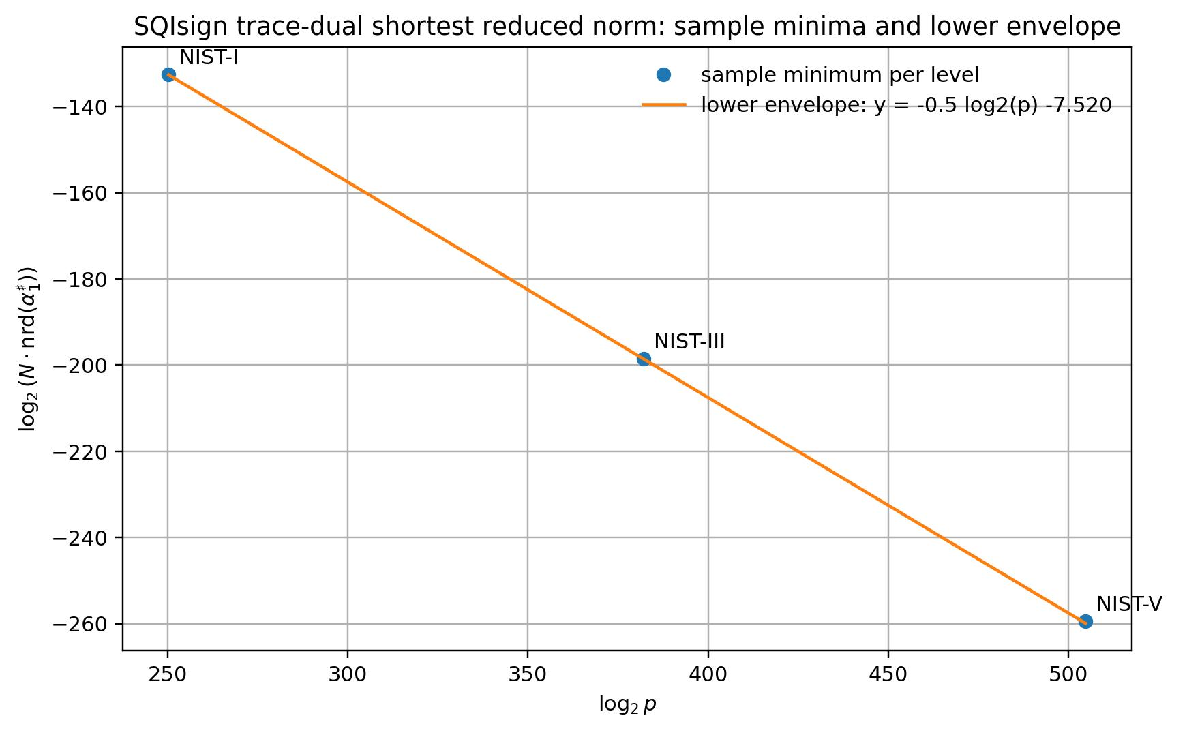
\includegraphics[width=\textwidth]{Figures/sqisign_trace_dual_transference_plot.pdf}
    \caption{Minimum over \(10{,}000\) samples of
    \(\log_2(D_{\mathrm{mix}}\operatorname{nrd}(\alpha_1^\#))\) for each NIST
    security level, where \(\alpha_1^\#\) is a shortest vector of the
    trace-dual lattice.}
    \label{fig:dual-norm}
\end{figure}